\documentclass[12pt]{article}

\usepackage{float} % improves positioning of figures and tables. i.e. [H]
\usepackage{gensymb} % Permits generic symbols like degree, ohm and such.
\usepackage{graphicx} % Required for inserting images
\usepackage[spanish,es-tabla]{babel}
\addto\captionsspanish{\renewcommand{\tablename}{Figura}}
\usepackage{amsmath} % permite ecuation*
\numberwithin{equation}{section} % for numbering equations using sections
\usepackage{listings} %permits use formal code listings in latex.
\usepackage{xcolor} % Optional, for custom colors
\usepackage{amsfonts} % For \mathbb
\usepackage{caption} % Para usar captions
\usepackage{pgfplots} % Plot para gráficar tipo matlab 3d
\pgfplotsset{compat=1.18}  % Plot para gráficar tipo matlab 3d
\decimalpoint % Asegura usar decimal point envez de coma
\usepackage{setspace} % Permite usar interlineado
\usepackage[margin=2.5cm]{geometry} % margenes 2.5 cm
\usepackage{newtxtext, newtxmath} % Times new roman
\usepackage{tabularx} % For tables with columns that automatically adjust width
\usepackage{fancyhdr} % permite la númeración de página
\pagestyle{fancy} % Activa el estilo fancy
\fancyhf{}                % clear default header and footer
\fancyfoot[R]{\thepage} % Pone el número de página en la esquina derecha (R) del pie de página (foot)
\usepackage{pdfpages} % To be able to include pdfs of the codes used
\usepackage[hidelinks]{hyperref} % for clickable refs
\usepackage{enumitem} % Fundamental para listas profesionales
\usepackage{mdframed}
\let\Bbbk\relax
\usepackage{amssymb}
\usepackage{hyperref}
\usepackage{tcolorbox}
\usepackage{listings}
\usepackage{xcolor}

\definecolor{codegreen}{rgb}{0,0.5,0}
\definecolor{codegray}{rgb}{0.5,0.5,0.5}
\definecolor{codepurple}{rgb}{0.58,0,0.82}
\definecolor{backcolour}{rgb}{0.97,0.97,0.97}

\lstdefinestyle{code}{
    backgroundcolor=\color{backcolour},
    basicstyle=\ttfamily\footnotesize,
    keywordstyle=\color{blue},
    commentstyle=\color{codegreen},
    stringstyle=\color{codepurple},
    numberstyle=\tiny\color{codegray},
    numbers=left,
    numbersep=5pt,
    breaklines=true,
    breakatwhitespace=false,
    showstringspaces=false,
    tabsize=4,
    frame=single,
    captionpos=b,
    literate={á}{{\'a}}1 {é}{{\'e}}1 {í}{{\'i}}1 {ó}{{\'o}}1 {ú}{{\'u}}1 {ñ}{{\~n}}1 {Á}{{\'A}}1 {É}{{\'E}}1 {Í}{{\'I}}1 {Ó}{{\'O}}1 {Ú}{{\'U}}1 {Ñ}{{\~N}}1
}
\lstset{style=code}

\newtcolorbox{pregunta}[1]{
  colback=blue!5!white,
  colframe=blue!75!black,
  title=Inciso (#1)
}

\newtcolorbox{pregunta2}[1]{
  colback=orange!5!white,
  colframe=orange!75!black,
  title=Inciso (#1)
}

\newtcolorbox{pregunta3}[1]{
  colback=green!5!white,
  colframe=green!75!black,
  title=Inciso (#1)
}

\newtcolorbox{pregunta4}[1]{
  colback=purple!5!white,
  colframe=purple!75!black,
  title=Inciso (#1)
}

\newtcolorbox{pregunta5}[1]{
  colback=yellow!5!white,
  colframe=yellow!75!black,
  title=Inciso (#1)
}



\title{ 

\includegraphics[width=10cm,height=10cm,keepaspectratio]{logoTec.png} 
\\
\vspace{1.5cm}
1er Mini-Proyecto Cuántica \\
}
\author{
Luis Daniel González Alcocer \small{A01286903@tec.mx} \\
Andrés Saul Pérez Martínez   \small{A01199376@tec.mx} \\
Andros Izhar Alvarado Sánchez \small {A00842107@tec.mx}
}
\date{
    \vspace{1.5cm}
\textbf{Profesor:} Julio César Gutiérrez Vega\\
\textbf{Curso:} Fundamentación de la electrodinámica (Gpo 601)\\
\vspace{1.5cm}
\today % Sets date
}

\begin{document}
\renewcommand{\tablename}{Tabla}
\maketitle
\newpage
\tableofcontents
\newpage

\section{Parte 1: Análisis dinámico del pozo infinito simétrico [45 puntos]}


\begin{pregunta}{1.}
\textbf{Cálculo de las amplitudes.} Aplicando la condición de normalización $\int_{-\infty}^{\infty} |\varphi_n(x)|^2 \, \mathrm{d}x = 1$, demuestren \textbf{analíticamente} que las amplitudes $A_n$ y $B_n$ en los eigenestados pares e impares del pozo finito simétrico están dadas por las Ecs. 18 y 19

\begin{equation}
A_n = \sqrt{\frac{q_n}{a q_n + 1}}, \qquad B_n = \frac{\cos k_n a}{\exp(-q_n a)} A_n, \tag{18}
\end{equation}
donde $k_n = (\pi/2a)\,\mu_n$ y $q_n = (\pi/2a)\sqrt{\mu_{\text{máx}}^2 - \mu_n^2}$. Para los eigenestados impares obtenemos
\begin{equation}
A_n = \sqrt{\frac{k_n}{a k_n - \tan(a k_n)}}, \qquad B_n = \frac{\sin k_n a}{\exp(-q_n a)} A_n. \tag{19}
\end{equation}
\end{pregunta}
%================================================================================
% INICIO PREGUNTA 1

El pozo finito simétrico tiene la siguiente función de potencial.
\begin{equation*}
U\left(x\right)=\left\{\begin{array}{ll}0, & \left|x\right|<a\\ U_0, & \left|x\right|>a\end{array}\right., \qquad U_0\in\mathbb{R}>0.
\end{equation*}

Para este pozo en particular, tenemos las siguientes soluciones dependiendo del intervalo en función de $k_n$ y $q_n$. Por ahora, analicemos los eigenestados pares.  
\textbf{Eigenestados pares} (simétricos)
\begin{equation*}
\varphi_n\left(x\right)=\left\{\begin{array}{lll}A_n\cos k_n x, & \left|x\right|<a, \qquad & k_n=\sqrt{2ME_n/\hbar^2},\\ B_n\exp\left(-q_n x\right), & x>a, \qquad & q_n=\sqrt{2M\left(U_0-E_n\right)/\hbar^2}.\end{array}\right.
\end{equation*}

Se inicia con la condición de normalización, que implica que la partícula debe estar en algún lugar en todo el espacio... 

\begin{equation}
    1 = \int_{-\infty}^{-a}B_n^2 \exp (2q_nx) \, dx 
    + \int_a^{\infty} B_n^2 \exp (-2q_nx) \, dx
    +2A^2_n \int_0^a\cos^2 (k_nx) \,dx
    \label{eq: norm:prob}
\end{equation}


Por simetría, las primeras dos integrales de ecuación \ref{eq: norm:prob} son simétrica y juntas dan un resultado de $B_n^2/q_n \exp (-2q_n a)$, mientras que la última integral se resuelve usando la identidad $\cos^2(k_nx)=\frac{1}{2}(1+\cos(2k_nx))$. Por lo que ecuación \ref{eq: norm:prob} se simplifica a:

\begin{equation}
    1= \frac{B^2_n}{q_n} \exp (-2q_na)+A_n^2\left(a+\frac{1}{2k_n}\sin(2ak_n)\right)
    \label{eq: A y B prob1}
\end{equation}


Para simplificar esto, se necesita una relación entre la variable $B_n$ y $A_n$. Dado que $\varphi_n$ debe ser continua, ambos deben valer lo mismo en $x=a$. Por lo que:

\begin{equation}
    A_n\cos(k_na)=B_n \exp(-q_na)
    \label{eq: cond front1}
\end{equation}

Ahora se reescribe \ref{eq: A y B prob1} en función de $A_n$ y se busca resolver para $A_n$.

\begin{align}
    1=&A_n^2\left(\frac{\cos^2(k_na)}{q_n}+a+\frac{1}{2k_n}\sin(2ak_n)\right) \\
    A_n^2 &= \frac{1}{\frac{\cos^2(ak_n)}{q_n} + a+\frac{1}{2k_n}\sin(2ak_n)}
\end{align}

Multiplicando por $q_n$ y utilizando la ecuación característica $\tan(ak_n)=\frac{q_n}{k_n}$, se puede llegar a la siguiente ecuación:

\begin{align}
    A_n^2 =& \frac{q_n}{\cos^2(k_na)+q_na+\sin^2(k_na)} \\
    A_n =& \sqrt{\frac{q_n}{1+q_na}} \label{eq: A par}
\end{align}

Donde la ecuación \ref{eq: A par} nos da el valor de $A_n$ para que este sea siempre normalizado. Ahora, para obtener $B_n$ se utiliza la ecuación \ref{eq: cond front1} y se llega a:
\begin{equation}
    B_n=\frac{\cos(k_na)}{\exp(-q_na)}A_n
\end{equation}

Ahora, se continua con los estados impares. 

\begin{itemize}
    \item \textbf{Eigenestados impares} (antisimétricos)
    \begin{equation}
        \varphi_n\left(x\right) = \left\{
        \begin{array}{lll}
            A_n \sin k_n x, & \qquad |x| < a, & \qquad k_n = \sqrt{2ME_n/\hbar^2}, \\
            B_n \exp\left(-q_n x\right), & \qquad x > a, & \qquad q_n = \sqrt{2M\left(U_0 - E_n\right)/\hbar^2}.
        \end{array}
        \right.
    \end{equation}
\end{itemize}

\textbf{Nota:} en la fuente original las definiciones de $k_n$ y $q_n$ para los eigenestados impares aparecen intercambiadas. Aquí se corrigen para que coincidan con las de los eigenestados pares, ya que $k_n$ corresponde a la región $|x|<a$ donde $U=0$, y $q_n$ a la región $|x|>a$ donde $U=U_0$.

Se inicia nuevamente con la condición de normalización, que lleva a:

\begin{equation}
    \frac{1}{2} = \int_0^a A_n^2 \sin^2(k_nx) \, dx + \int_a^{\infty} B_n^2 \exp(-2q_nx) \, dx
\end{equation}

\begin{equation}
    \frac{1}{2} = \frac{1}{2}\left[A_n^2 \int_0^a \left(1-\cos(2k_nx)\right) dx + \frac{B_n^2}{q_n}\exp(-2q_nx)\Big|_{\infty}^{a}\right]
\end{equation}

\begin{equation}
    1 = A_n^2\left[a-\frac{\sin(2k_na)}{2k_n}\right] + \frac{B_n^2}{q_n}\exp(-2q_na)
    \label{eq: norm impar}
\end{equation}

Ahora, se usa nuevamente la condición de frontera:

\begin{equation}
    A_n\sin(k_na) = B_n\exp(-q_na)
    \label{eq: cond front impar}
\end{equation}

Por lo que ahora en términos de $A_n$ \ref{eq: norm impar} se vuelve:

\begin{align}
    1 =& A_n^2\left[a-\frac{\sin(2k_na)}{2k_n}+\frac{\sin^2(k_na)}{q_n}\right] \\
    A_n^2 =& \frac{1}{a-\frac{\sin(2k_na)}{2k_n}+\frac{\sin^2(k_na)}{q_n}}
    \label{eq: A2 impar}
\end{align}

Para simplificar \ref{eq: A2 impar} se utiliza la ecuación maestra:

\begin{equation}
    \cot(k_na) = -\frac{q_n}{k_n}
    \label{eq: ec maestra impar}
\end{equation}

Usando \ref{eq: ec maestra impar} y multiplicando por $q_n$ \ref{eq: A2 impar}, se llega a:

\begin{align}
    A_n^2 =& \frac{q_n}{aq_n+\cos^2(k_na)+\sin^2(k_na)} \\
    A_n =& \sqrt{\frac{q_n}{aq_n+1}} \label{eq: A impar}
\end{align}

Por lo que $B_n$ llega de \ref{eq: cond front impar}:

\begin{equation}
    B_n = \frac{\sin(k_na)}{\exp(-q_na)}A_n
    \label{eq: B impar}
\end{equation}

Quedando entonces demostrado el cálculo de las amplitudes.


 %================================================================================
\begin{pregunta}{2.}
\textbf{Cálculo de las eigenenergías y estados estacionarios.} Elabora una rutina computacional para encontrar las eigenenergías $E_n$ en un pozo finito. Para fines numéricos, consideren las constantes $\hbar = 1$, semi-ancho del pozo $a = 1$, y masa $M = \pi^2/8$. Estos valores están pensados para que la energía basal del pozo infinito [Ec. (15)] sea $V_0 = 1$. Como ejemplo concreto, para la profundidad del pozo toma $U_0 = 110$.
 
Programa una función que evalúe los eigenestados $\varphi_n(x)$ del pozo finito.
 
\textbf{Para el reporte:}
 
$\rightarrow$ Tabulen los valores de todas las energías permitidas en el pozo.
 
$\rightarrow$ Grafiquen los primeros 8 eigenestados $\varphi_n(x)$ del pozo. Corroboren que entre más grande es la energía, el eigenestado penetra más en la región clásicamente \textit{prohibida}, es decir, donde $|x| > a$. Asegúrense de usar las amplitudes $A_n$ y $B_n$ analíticas para que sus eigenestados estén normalizados automáticamente. Para tener un indicio de que las cosas están correctas, verifiquen usando diversas parejas de eigenestados que se cumple la ortonormalidad
\begin{equation}
\int_{-\infty}^{\infty} \varphi_p^{*}(x) \, \varphi_q(x) \, \mathrm{d}x = \delta_{pq}. \tag{1}
\end{equation}
Esta integral puede hacerse con la regla del trapecio si muestrean la coordenada $x$ con suficiente resolución y tomando un intervalo lo suficientemente grande para asegurarse que las exponenciales han decaído prácticamente a cero. Así el error de truncamiento es despreciable.
\end{pregunta}

\subsection*{Sobre el código:}

El código se puede ver en el apéndice. Véase el Apéndice \ref{ap: sec1prob2}. Ahora sí, continuemos con el problema.
\\ 

Primero, se muestra en la Tabla \ref{tab:energies} los distintos valores de las energías encontrados al resolver la ecuación maestra. Como el pozo es finito, hay un finito de energías permisibles para estados atrapados. En este caso, se obtienen $11$ eigenenergías. 
\begin{table}[h]
\centering
\begin{tabular}{cccc}
\hline
$n$ & Even energies & $n$ & Odd energies \\
\hline
1 & 0.8887 & 2& 3.5531 \\
3 & 7.9880 & 4& 14.1841 \\
5 & 22.1268 & 6& 31.7943 \\
7 & 43.1531 & 8& 56.1502 \\
9 & 70.6928 & 10& 86.5879 \\
11 & 103.2200 &--& -- \\
\hline
\end{tabular}
\caption{Tabulación de los estados de energía para los estados tanto pares e impares. Se muestra en este caso 6 energías para los estados pares y 5 para los impares.}
\label{tab:energies}
\end{table}


Asimismo, en la Figura \ref{fig:eigenenergies}, se puede ver de una forma gráfica las energías, en comparación al pozo finito. Se observa que al inicio, están muy juntas mientras que las últimas están muy cerca del fin del pozo. 

Se espera que los eigenestados con energías bajas se parezcan a los eigenestados del pozo infinito, mientras que los eigenenergias con energías altas tengan una alta penetración en el pozo.
\begin{figure}
    \centering
    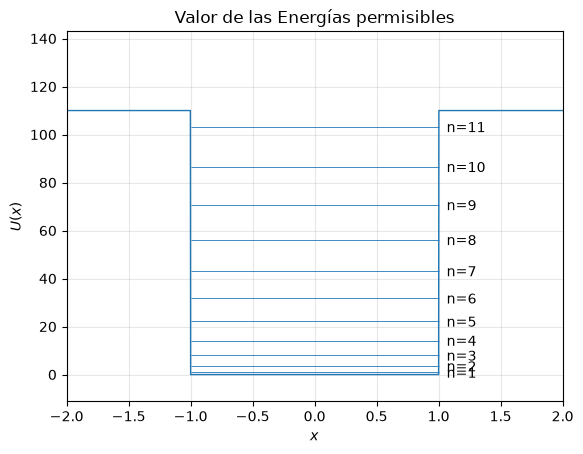
\includegraphics[width=0.75\linewidth]{mini1/energiaspermisibles.png}
    \caption{Se muestran como rayas todas las energías permitidas en el pozo. Para los valores específicos de $a=1, U_0=110, V_0=1, M=\frac{\pi^2}{8}$, obtuvieron 11 energías. Se observa que la separación entre cada energía va aumentando conforme aumenta el nivel.}
    \label{fig:eigenenergies}
\end{figure}

En la Figura \ref{fig:eigenestados}, se pueden observar los primeros 8 eigenestados del pozo finito. Como se esperaba, los primeros eigenestados, se parecen al pozo infinito, dado que casi no se llega a penetrar la pared. En cambio, los estados grandes este efecto es más notorio. Ahora, lo último que queda es checar la ortonormalidad de las ecuaciones. Se realiza la siguiente integral de manera computacional:

\begin{equation}
\int_{-\infty}^{\infty} \varphi_p^{*}(x) \, \varphi_q(x) \, \mathrm{d}x = \delta_{pq}. 
\label{eq:ortonormality}
\end{equation}
\begin{figure}
    \centering
    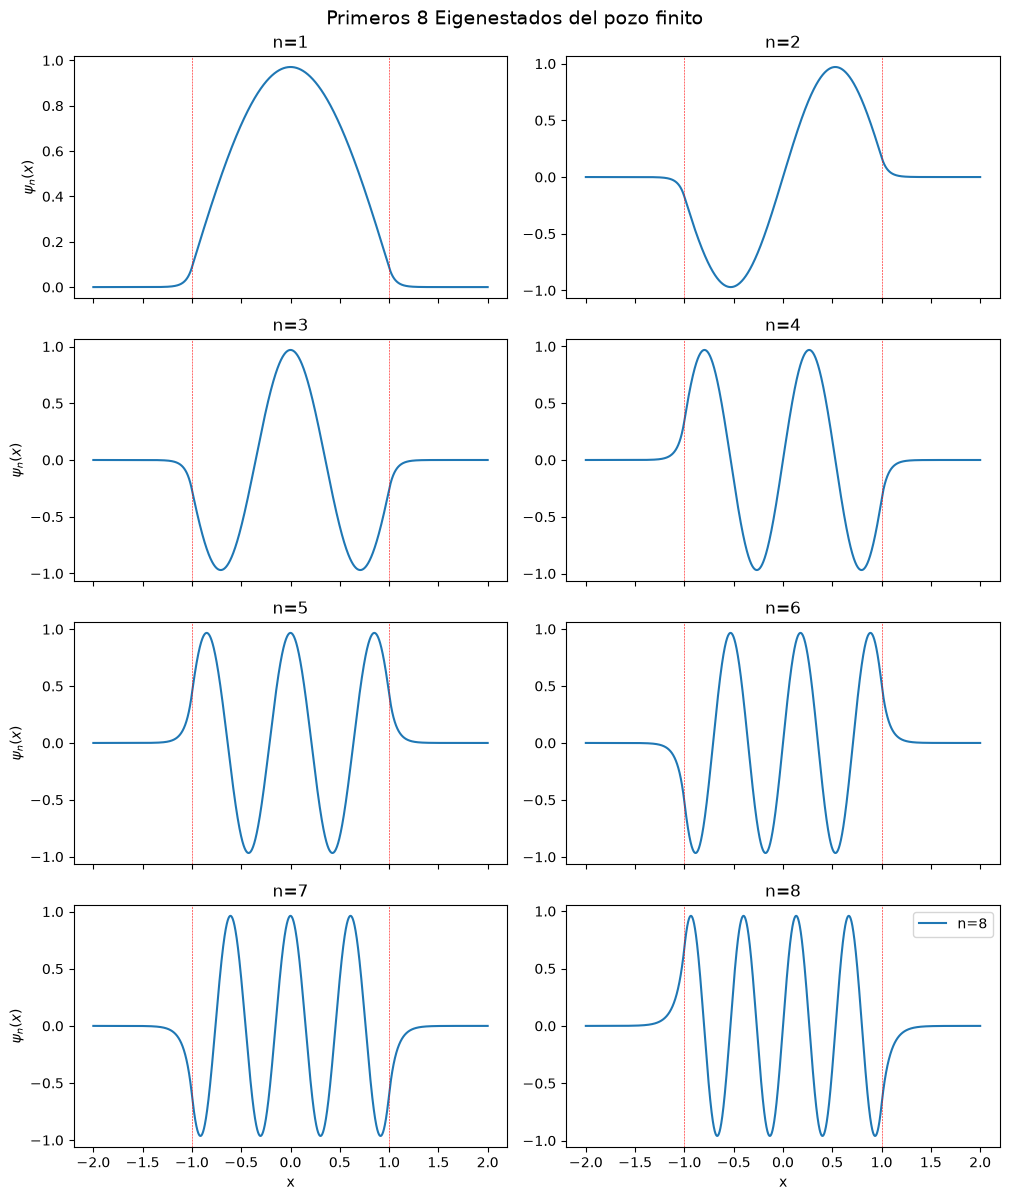
\includegraphics[width=0.75\linewidth]{eigenestados.png}
    \caption{Los eigenestados de las primeras 8 energías del pozo. Se observa que están todas entre el rango de -1 a 1, que debe ser así para ser normalizadas. En la región del pozo, se muestran oscilaciones de senos o cosenos, mientras que después del pozo se observan exponenciales por la zona prohibida. Para energías altas, se llega a penetrar más en la zona prohibida.}
    \label{fig:eigenestados}
\end{figure}


Ahora, para poder ver que realmente los eigenestados son ortonormales, utilizamos una matriz de traslape $S$ en el cual sus entradas se definen de la siguiente manera:

\begin{equation}
    S_{ij} = \int_{-\infty}^{\infty} \varphi_i^{*}(x) \, \varphi_j(x) \, \mathrm{d}x
\end{equation}

El resultado de $S$ se puede apreciar en la Figura \ref{fig:overlaps}. Claramente aquí se demuestra la ortogonalidad dado que representa una matriz identidad, que es equivalente a la delta de Dirac que se utiliza en la ecuación \ref{eq:ortonormality}.


\begin{figure}
    \centering
    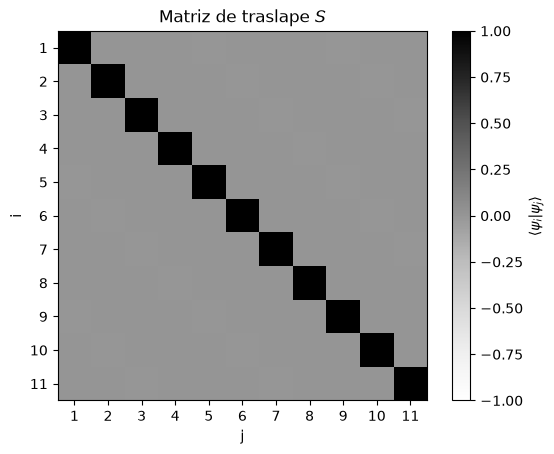
\includegraphics[width=0.75\linewidth]{overlapS.png}
    \caption{La matriz de traslape $S$ que muestra la ortonormalidad de los eigenestados. Como solamente la diagonal principal contiene valores no nulos, se muestra la ortogonalidad. Asimismo, como esta tiene una diagonal de 1's, vemos que está también normalizada y por lo tanto los eigenestados son ortonormales.}
    \label{fig:overlaps}
\end{figure}





 
\begin{pregunta}{3.}
\textbf{Evolución temporal.} En el problema anterior hemos encontrado la base de eigenestados ortogonales del pozo finito, las funciones $\varphi_n(x)$, donde $n = \{1, 2, \ldots, N\}$ con $N$ siendo el máximo número de eigenestados atrapados en el pozo. Programen una rutina computacional para simular la evolución temporal de una función de onda inicial $\phi(x,0) = f(x)$ dentro del pozo finito de potencial. Como base del algoritmo, usen la expansión estándar en términos de eigenestados
\begin{equation}
\phi(x,t) = \sum_{n=1}^{N} c_n \varphi_n(x) \exp(-\mathrm{i}\omega_n t), \qquad \omega_n = \frac{E_n}{\hbar}, \tag{2}
\end{equation}
donde $\varphi_n(x)$ es el $n$-ésimo estado estacionario del sistema cuya eigenenergía es $E_n$. Los coeficientes $c_n$ dependen de la forma inicial de la función de onda, en general
\begin{equation}
c_n = \int_{-\infty}^{\infty} \varphi_n^{*}(x) f(x) \, \mathrm{d}x. \tag{3}
\end{equation}
 
\begin{enumerate}
\item[a)] Simulen la evolución de una función de onda inicial dada por
\begin{equation}
\phi(x,0) = A \left[ \varphi_1(x) + 0.7\varphi_2(x) - \mathrm{i}1.2\varphi_3(x) + (2 - \mathrm{i})\varphi_4(x) \right], \tag{4}
\end{equation}
donde $A$ es la constante de normalización (calcúlenla previamente).
 
\textbf{Para el reporte:}
 
$\rightarrow$ Generen una gráfica bidimensional de la función de densidad de probabilidad $|\phi(x,t)|^2$.
 
$\rightarrow$ Grafiquen el valor esperado de la posición en función del tiempo.
 
\item[b)] \textbf{Pulso Gaussiano.} Consideren el pulso Gaussiano de ancho $2b$ centrado en $x = c$
\begin{equation}
\phi(x,0) = f(x; b, c) = A \exp\left[ -\frac{(x-c)^2}{b^2} \right] \exp\left( \mathrm{i}\frac{M v_0}{\hbar} x \right), \tag{5}
\end{equation}
donde $A$ es la constante de normalización. Consideremos que la anchura $2b$ es lo suficientemente pequeña para que la función Gaussiana prácticamente sea cero en las paredes $x = \pm a$. El pulso de la Ec. (5) tiene velocidad inicial $v_0$ en $t = 0$, es decir, un momentum inicial $p_0 = M v_0$.
 
\textbf{Para el reporte:}
 
$\rightarrow$ Calculen \textbf{analíticamente} la constante de normalización $A$.
 
Para las simulaciones que siguen tomen $b = 0.2$ y $c = 0.4$. Simulen la evolución del pulso de la Ec. (5) en el pozo finito. Consideren exclusivamente los $N$ eigenestados atrapados $\varphi_n(x)$ del pozo finito para hacer la expansión.
 
$\rightarrow$ Generen una gráfica bidimensional de la función de densidad de probabilidad $|\phi(x,t)|^2$.
 
$\rightarrow$ Grafiquen el valor esperado de la posición en función del tiempo $\langle x \rangle$.
 
$\rightarrow$ Hagan un video de la evolución del pulso. Importante: Formato mp4.
 
\textbf{Consideraciones físicas a tomar en cuenta:} Es importante notar que para expandir el pulso inicial $f(x)$ solo tenemos un número finito de eigenestados atrapados $\varphi_n(x)$ del pozo finito. En general la base finita de estados $\varphi_n(x)$ no será una base completa para expandir cualquier función arbitraria $f(x)$ inicial del pozo. Supongamos que $g(x)$ sea la función aproximada de $f(x)$ usando la base finita, $g(x) = \sum_{n=1}^{N} c_n \varphi_n(x)$. La evolución de $g(x)$ preserva energía ya que se puede descomponer de manera exacta en eigenestados del sistema. Pero esto no va a ocurrir con la función exacta $f(x)$, ya que una parte de la función no puede reconstruirse con la base finita de los estados atrapados $\varphi_n(x)$. La consecuencia física de esto es que cuando el pulso $f(x)$ evoluciona dentro del pozo una parte de su energía se disipará por las paredes como ondas viajeras que se alejan del pozo. En un tiempo largo, el pulso que quede dentro del pozo corresponderá a una función que puede construirse exclusivamente con los eigenestados $\varphi_n(x)$. La analogía de este problema en óptica corresponde a la pérdida de energía de un pulso de luz en el acoplamiento de una fibra óptica. La reconstrucción completa de la función $f(x)$ podría hacerse usando la superposición finita de estados atrapados [lo cual nos da la función $g(x)$] más una superposición continua de ondas viajeras con energía mayor a $U_0$ [lo cual nos da el complemento $f(x) - g(x)$].
\end{enumerate}
\end{pregunta}
 
\begin{pregunta}{4.}
En clase analizamos el potencial escalón definido por
\begin{equation}
U(x) = \begin{cases} 0, & x < 0 \\ U_0, & x \geq 0 \end{cases}, \qquad U_0 \in \mathbb{R} > 0. \tag{6}
\end{equation}
El estado $\phi(x)$ con energía $E$ está dado por
\begin{equation}
\phi(x) = \begin{cases} A \exp(\mathrm{i}kx) + B \exp(-\mathrm{i}kx), & x \leq 0, \qquad k = \sqrt{\dfrac{2ME}{\hbar^2}}, \\[2ex] C \exp(-qx), & x > 0, \qquad q = \sqrt{\dfrac{2M}{\hbar^2}(U_0 - E)}, \end{cases} \tag{7}
\end{equation}
donde $A$, $B$, $C$ son las amplitudes de las ondas incidente, reflejada y transmitida, respectivamente. Como el estado no está atrapado, la energía $E$ de la partícula es un parámetro libre dentro del intervalo $0 < E < U_0$. En clase encontramos que las amplitudes relativas de la onda reflejada y transmitida con respecto a la incidente son
\begin{align}
\frac{B}{A} &= \frac{k - \mathrm{i}q}{k + \mathrm{i}q} = \exp(\mathrm{i}\gamma), \qquad \text{donde} \qquad \gamma = -2\arctan\left( \frac{q}{k} \right), \tag{8} \\
\frac{C}{A} &= \frac{2k}{k + \mathrm{i}q}. \tag{9}
\end{align}
La fase $\gamma$ representa el desfasamiento de la onda reflejada con respecto a la incidente al momento de la reflexión en la pared.
 
\begin{enumerate}
\item[a)] Consideren ahora el pozo finito de potencial simétrico y encuentren una ecuación característica unificada (es decir, que sirva para estados pares e impares) para los eigenvalores de energía. Para esto consideren que un estado estacionario dentro del pozo resulta de la superposición de dos estados viajeros contrapropagantes de la forma $\exp(\pm \mathrm{i}kx)$. Cuando la onda incidente se refleja en una pared del pozo sufre un corrimiento de fase $\gamma$. Un ciclo completo dentro del pozo incluye la reflexión en las dos paredes y el doble tránsito de la onda a lo largo del pozo. La condición de resonancia y reproducibilidad implica que el desfase total en un ciclo completo en la cavidad sea un múltiplo entero de $2\pi$. Pueden usar esta condición dinámica para deducir la ecuación característica unificada.
 
\item[b)] Evalúen la ecuación característica que obtuvieron en el inciso (a) con los datos numéricos de los incisos anteriores y demuestren que las eigenenergías son coincidentes.
\end{enumerate}
\end{pregunta}
 

\section{Parte 2: Análisis dinámico del pozo finito asimétrico [50 puntos]}
 
Consideremos ahora el pozo finito asimétrico definido por el potencial
\begin{equation}
U(x) = \begin{cases} U_1, & x < 0, \\ 0, & 0 \leq x < L, \\ U_2, & x \geq L, \end{cases} \qquad \{U_1, U_2\} > 0, \qquad U_2 \geq U_1, \qquad c \equiv \frac{U_2}{U_1} \geq 1, \tag{10}
\end{equation}

\begin{figure}
    \centering
    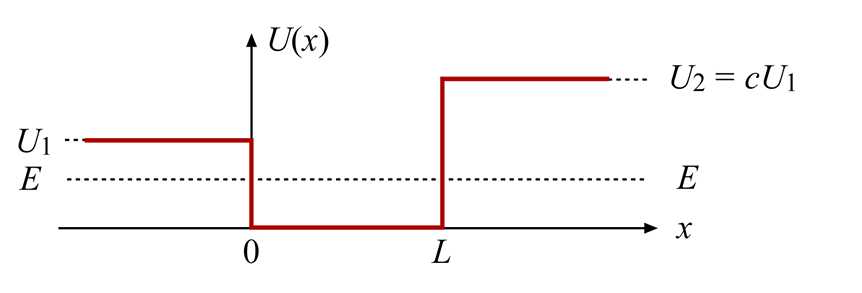
\includegraphics[width=0.5\linewidth]{mini1/pozo antisimétrico.png}
    \caption{Pozo infinito de potencial de anchura $L$ y paredes con potenciales diferentes}
    \label{fig:1}
\end{figure}
que se muestra en la Fig. 1. Sin perder generalidad, asumimos que $U_2 \geq U_1$, por lo que el factor de proporcionalidad $c \geq 1$. El factor $c$ se considera como un parámetro de asimetría entre ambas paredes. Observen que el pozo está definido entre $x = 0$ y $x = L$, pues al no ser simétrico, ya no tiene ninguna ventaja definirlo simétricamente alrededor de $x = 0$. Definimos el inicio del pozo en $x = 0$ para facilitar evaluaciones en esa frontera.
 
\begin{pregunta}{1.}
Escribe la forma general de las eigenfunciones $\varphi_n(x)$ del pozo asimétrico. Nota que el pozo tiene tres secciones de potencial constante. Asume que la energía de la partícula está en el rango $0 < E < U_1$. Observa que el pozo no tiene simetría, por lo que los estados $\varphi_n(x)$ no tienen paridad, como sí existía en el potencial simétrico. Esto último va a tener un impacto en la forma en la que escribas la forma del estado en la zona central de atrapamiento.
\end{pregunta}


% Figura del pozo (dibujo a mano): U_1 para x<0, 0 en 0<=x<L, U_2 para x>=L, nivel E por debajo de U_1
\begin{equation*}
U_2 = cU_1, \qquad c = \frac{U_2}{U_1} \geq 1, \qquad 0 \leq E \leq U_1 \leq U_2
\end{equation*}

Se observa que son tres áreas con potencial finito... La onda debe cumplir la ec. de Schrödinger $\forall x$
\begin{equation*}
-\frac{\hbar^2}{2m}\partial^2_x\varphi_ + V\varphi = E\varphi
\end{equation*}

Para $0<x<L$: $E - V = E$, dado que $V=0$.
\begin{equation*}
\Rightarrow -\frac{\hbar^2\partial^2\varphi}{2m} = E\varphi \Rightarrow \varphi = A\cos(\omega x) + B\sin(\omega x) \quad \text{donde} \quad \omega \equiv \sqrt{\frac{2mE}{\hbar^2}}
\end{equation*}

Para $x<0$: Si $U_1 - E > 0$
\begin{equation*}
\Rightarrow \partial^2\varphi = \frac{2m}{\hbar^2}(-E+U_1)\varphi = \kappa^2\varphi, \qquad \kappa \equiv \sqrt{\frac{2m(U_1-E)}{\hbar^2}}, \qquad \kappa > 0 \ldots
\end{equation*}
\begin{equation*}
\Rightarrow \varphi = C_1 e^{\kappa x} + C_2 e^{-\kappa x}
\end{equation*}
Claramente, el segundo término no es normalizable para $x<0$, por lo que $C_2 = 0$. Sea $C_1 = C$
\begin{equation*}
\Rightarrow \varphi(x) = C e^{+\kappa x}
\end{equation*}

Para $x>L$: $U_2 - E > 0$. Similar al pasado sea
\begin{equation*}
\gamma \equiv \sqrt{\frac{2m(U_2-E)}{\hbar^2}} = \sqrt{\frac{2m(cU_1-E)}{\hbar^2}}
\end{equation*}
\begin{equation*}
\Rightarrow \varphi = De^{-\gamma x}
\end{equation*}

Ahora, juntamos las soluciones para formar una solución continua.
\begin{equation}
\varphi(x) = \begin{cases} C e^{+\kappa x}, & x<0, \\ A\cos(\omega x) + B\sin(\omega x), & 0 \leq x < L, \\ De^{-\gamma x}, & x \geq L. \end{cases}
\label{eq: phi cases asim}
\end{equation}

Como el potencial no es simétrico, los estados $\varphi_n(x)$ no tienen paridad definida, por lo que en la zona central se conservan ambos términos, $\cos(\omega x)$ y $\sin(\omega x)$, con $A$ y $B$ en general distintos de cero. Las constantes $\omega$, $\kappa$ y $\gamma$ dependen de $E_n$.


 
\begin{pregunta}{2.}
Encuentra la ecuación característica para las eigenenergías $E_n$ de los estados estacionarios $\varphi_n(x)$ de una partícula atrapada en el potencial de pozo asimétrico. \textit{Hint: Puedes intentar la estrategia del problema 4 de la parte 1 del pozo simétrico. Opcionalmente, puedes parametrizar como lo hicimos en clase para que la ecuación quede más compacta y dependa solo de un parámetro.}
\end{pregunta}



Ahora las constantes $A,B,C,D$ de $\varphi(x)$ en la ecuación \ref{eq: phi cases asim} se calculan. Estas soluciones y sus derivadas deben coincidir en las condiciones de frontera \dots

\noindent En $x=0$:
\begin{equation*}
\boxed{C = A}, \qquad C\kappa = B\omega, \qquad \boxed{B = +\frac{\kappa}{\omega}C}
\end{equation*}

\noindent En $x=L$:
\begin{align*}
A\cos(\omega L) + B\sin(\omega L) &= De^{-\gamma L} \\
-A\omega\sin(\omega L) + B\omega\cos(\omega L) &= -D\gamma e^{-\gamma L}
\end{align*}

Remplazando a $A$ y $B$ en términos de $C$ \dots

\begin{align}
C\cos(\omega L) + \frac{\kappa}{\omega}C\sin(\omega L) &= De^{-\gamma L} \label{C1} \\
-C\omega\sin(\omega L) + \kappa C\cos(\omega L) &= -D\gamma e^{-\gamma L} \label{C2}
\end{align}

Multiplicando por $\kappa$ \ref{C1} y luego restando a \ref{C2}
\begin{equation*}
\frac{\kappa^2}{\omega}C\sin(\omega L) + C\omega\sin(\omega L) = D[\kappa+\gamma]e^{-\gamma L}
\end{equation*}
\begin{equation*}
C\sin(\omega L)\left[\frac{\kappa^2}{\omega} + \omega\right] = De^{-\gamma L}[\kappa+\gamma]
\end{equation*}
\begin{equation*}
\boxed{D = C e^{\gamma L} \left[\frac{\sin(\omega L)\left[\kappa^2 + \omega^2\right]}{\omega[\gamma+\kappa]}\right]}
\end{equation*}

Ahora, ya tenemos todas las constantes en términos de $C$. Sin embargo de las ecuaciones \ref{C1}, \ref{C2}, podemos también obtener una ecuación que relacione las variables $\omega, \gamma, \kappa$, lo que nos permitiría obtener los estados de energía permisibles.

Multiplicando \ref{C1} por $\gamma$ y despejando $\frac{D}{C}e^{-\gamma L}\gamma$
\begin{equation*}
\frac{D}{C}\gamma e^{-\gamma L} = \gamma\cos(\omega L) + \frac{\kappa}{\omega}\gamma\sin(\omega L) = -\kappa\cos(\omega L) + \omega\sin(\omega L)
\end{equation*}
\begin{equation*}
\Rightarrow \gamma\cos(\omega L) + \frac{\kappa}{\omega}\gamma\sin(\omega L) = -\kappa\cos(\omega L) + \omega\sin(\omega L)
\end{equation*}
\begin{equation*}
\cos(\omega L)\left[\gamma + \kappa\right] = \sin(\omega L)\left[\omega - \frac{\kappa\gamma}{\omega}\right]
\end{equation*}
\begin{equation*}
\Rightarrow \tan(\omega L) = \frac{\gamma + \kappa}{\omega - \frac{\kappa\gamma}{\omega}} = \frac{\omega(\gamma+\kappa)}{\omega^2 - \kappa\gamma}
\end{equation*}
\begin{equation}
\boxed{\tan(\omega L) = \frac{\omega(\kappa+\gamma)}{\omega^2 - \kappa\gamma}} \qquad \leftarrow \text{Ecuación Maestra}
\end{equation}

Recordando
\begin{equation*}
\kappa = \sqrt{\frac{2m(U_1-E)}{\hbar^2}}, \qquad \omega = \sqrt{\frac{2mE}{\hbar^2}}, \qquad \gamma = \sqrt{\frac{2m(cU_1-E)}{\hbar^2}}
\end{equation*}

Notemos que
\begin{equation*}
-\kappa^2 + \gamma^2 = \frac{2mcU_1}{\hbar^2} - \frac{2mU_1}{\hbar^2} = \frac{2mU_1}{\hbar^2}(c-1)
\end{equation*}
\begin{equation*}
\kappa^2 + \omega^2 = \frac{2mU_1}{\hbar^2}, \qquad \gamma^2 + \omega^2 = \frac{2mcU_1}{\hbar^2}
\end{equation*}

Usando estas ecuaciones, sea $z \equiv \omega L$ una variable adimensional
\begin{equation*}
\Rightarrow z^2 + (\kappa L)^2 = \frac{2mU_1L^2}{\hbar^2}
\end{equation*}
\begin{equation*}
\therefore z_{max} = \frac{L}{\hbar}\sqrt{2mU_1}
\end{equation*}

Usando $z_{max}$, escribimos $\kappa$ y $\gamma$ en términos de $z$
\begin{equation*}
z^2 + (\kappa L)^2 = z_{max}^2
\end{equation*}
\begin{equation*}
\Rightarrow \boxed{\kappa L = \sqrt{z_{max}^2 - z^2}}
\end{equation*}
\begin{equation*}
(L\gamma^2) + (\omega L)^2 = \frac{2mcU_1L^2}{\hbar^2}
\end{equation*}
\begin{equation*}
z^2 + (L\gamma)^2 = cz_{max}^2
\end{equation*}
\begin{equation*}
\boxed{\Rightarrow L\gamma = \sqrt{cz_{max}^2 - z^2}}
\end{equation*}

Ahora, se reescribe la ecuación maestra, multiplicando y dividiendo por $L^2$...
\begin{equation}
\boxed{\tan(z) = \frac{z\sqrt{z_{max}^2 - z^2} + z\sqrt{cz_{max}^2 - z^2}}{z^2 - \sqrt{z_{max}^2 - z^2}\sqrt{cz_{max}^2 - z^2}}}
\end{equation}



 
\begin{pregunta}{3.}
Deduce una expresión cerrada para el número total $N$ de estados estacionarios atrapados $\varphi_n(x)$ que el pozo soporta dados los parámetros $U_1$, $U_2$ y $L$.
\end{pregunta}
 
\begin{pregunta}{4.}
El pozo finito simétrico siempre soporta al menos un estado atrapado, sin importar lo estrecho o poco profundo que sea. ¿Es lo mismo para el pozo asimétrico? ¿Pueden darse las condiciones para que el pozo asimétrico no soporte ningún estado? De ser así, ¿cuál es la condición de corte para no tener estados atrapados en el pozo?
\end{pregunta}
 
\begin{pregunta}{5.}
Una vez que las eigenenergías $E_n$ han sido determinadas, las amplitudes de las funciones en cada segmento del potencial se pueden encontrar de forma algebraica cerrada (similarmente al caso de las Ecs. (18) y (19) del pozo simétrico). Usando la condición de normalización de $\varphi_n(x)$ y las conexiones entre las amplitudes de las funciones en cada segmento, determina analíticamente las amplitudes. Simplifica todo lo que se pueda.
\end{pregunta}

% Creo que está mal dado que se nos pide utilizar las eigenenergías, pero pues no lo quise borrar.
Por lo que se prosigue a realizar la normalización...

\begin{equation*}
\int_{-\infty}^{\infty}\varphi'(x)\varphi(x)dx = 1 \Rightarrow \frac{1}{C} = \int_{-\infty}^{0} e^{+\kappa x}\,dx + \int_{0}^{L}\left[\cos(\omega x) + \frac{\kappa}{\omega}\sin(\omega x)\right]dx + \int_{L}^{\infty}\beta e^{\gamma L} e^{-\gamma x}\,dx
\end{equation*}
donde
\begin{equation*}
\beta \equiv \left[\frac{\sin(\omega L)\left[\kappa^2+\omega^2\right]}{\omega[\gamma+\kappa]}\right]
\end{equation*}
\begin{equation*}
\Rightarrow \frac{1}{C} = \frac{1}{\kappa} + \left[\frac{1}{\omega}\sin(\omega x) - \frac{\kappa}{\omega^2}\cos(\omega x)\right]_0^L + \frac{\beta}{\gamma}
\end{equation*}
\begin{equation*}
\frac{1}{C} = \frac{1}{\kappa} + \left[\frac{1}{\omega}\sin(\omega L) + \frac{\kappa}{\omega^2}\big(1 - \cos(\omega L)\big)\right] + \frac{\beta}{\gamma}e^{-\gamma L}
\end{equation*}
\begin{equation*}
\boxed{C = \left[\frac{1}{\kappa} + \frac{1}{\omega}\sin(\omega L) + \frac{\kappa}{\omega^2}\big(1-\cos(\omega L)\big) + \frac{\beta}{\gamma}e^{-\gamma L}\right]^{-1}}
\end{equation*}


 
\begin{pregunta}{6.}
Ahora toca evaluar numéricamente los resultados analíticos obtenidos anteriormente. Considera los parámetros similares al caso simétrico de la Parte 1. Es decir, $\hbar = 1$, ancho del pozo $L = 2$, y masa $M = \pi^2/8$. Para la profundidad del pozo tomen $U_1 = 85$ y $U_2 = cU_1$, donde $c \geq 1$.
 
\begin{enumerate}
\item[a)] Encuentra las energías del pozo cuando $c = 2$.
 
\item[b)] Grafica los eigenestados correspondientes.
 
\item[c)] Hagan el inciso 3(b) de la Parte 1 sobre la propagación de un pulso Gaussiano, pero ahora con el potencial asimétrico.
\end{enumerate}
 
\textit{Sugerencia: Verifiquen que sus resultados analíticos obtenidos para el pozo asimétrico se reducen al caso del pozo simétrico cuando $c = 1$.}
\end{pregunta}
 

\appendix
\section{Códigos de problema 1 Inciso 2} \label{ap: sec1prob2}
Se utilizó Python y se usó la IA mayormente para resolver dudas y graficar de mejor manera. Todo el código y lógica fue hecho por los autores y estos se hacen responsables de su veracidad.

\begin{lstlisting}[language=Python, caption={Problema 1 Inciso 2.}]
import numpy as np
from scipy.optimize import brentq
import matplotlib.pyplot as plt
from matplotlib.ticker import MultipleLocator

def energias_permisibles(mumax: float,*,eps=1e-12,a=1,hhbar=1,M=1/8 * np.pi**2) -> np.ndarray:
    '''
    Se calcula las energías permisibles para el pozo finito. Se sabe que la función tan(pi/2 * x),
    tiene polos en los valores pares de x y siempre es positivo en el intervalo 2n, 2n+1.

    Args:
        mumax:      the maximum value of mumax. (sqrt(U0/V0))
        eps:        a small tolerance parameter
        a:          width of the finite well
        hbar:       the value of Planck reduced constant
        M:          the mass of the particle
    returns:
        Tuple(array,array) with even and odd energies respectively.

    '''
    f = lambda x: x*np.sin(np.pi*x/2) - np.sqrt(mumax**2 - x**2)*np.cos(np.pi*x/2)
    g = lambda x:  np.sqrt(mumax**2 - x**2)*np.sin(np.pi*x/2) +x*np.cos(np.pi*x/2)
    raicespar = []
    raicesimpar = []
    n = 0
    while 2*n < mumax:
        #estados pares
        low = 2*n + 1e-12
        high = min(2*n + 1-eps, mumax)
        if f(low)*f(high) < 0:
            raicespar.append(brentq(f, low, high))
        #estados impares
        low+=1; high= min(high+1,mumax)
        if low>mumax:
            n+=1
            break
        if g(low)*g(high) < 0:
            raicesimpar.append(brentq(g,low,high))
        n += 1
    E1 = (hbar*np.pi)**2/(2*M*(2*a)**2)    
    x_par, x_imp = np.array(raicespar),np.array(raicesimpar)
    energias = (E1*x_par**2, E1*x_imp**2)
    return energias





def plot_energies(energias,*,a=1,ax=None): 
    '''
    Plots allowed energie levels in horizontal lines.
    
    Args:
        energias:       array(s) that contain the energies
        a:              width of the well
        ax:             if included, the axis for graph
    Raises:
        Value error if energies is empty.
    '''
    energias =  np.sort(np.concatenate(energias))
    if len(energias) ==0:
        raise ValueError("Energías must at least have 1 value.")
    if ax is None:
        _, ax = plt.subplots()

    for (index,e) in enumerate(energias,start=1):
        ax.text(1, e, f"  n={index}", va="center_baseline")
    for e in energias:
        plt.hlines(e,-a,a,lw=0.6)
    plt.ylabel("Energía") 
    ax = graph_well(ax)
    plt.title("Valor de las Energías permisibles")
    plt.show()

def graph_well(ax,*,a=1,U0=110):
    def potential(x: np.ndarray, *, a: float, U0: float) -> np.ndarray:
        """
        Helper function that returns 0 for |x| <= a and U0 otherwise.

        Args:
            x: Positions at which to evaluate the potential.
            a: Half-width of the well.
            U0: Potential height outside the well.

        Returns:
            Array of potential values with the same shape as x.
        """
        return np.where(np.abs(x) <= a, 0.0, U0)
    steps = 2001
    x = np.linspace(-2 * a, 2 * a, steps)
    y = potential(x, a=a, U0=U0)

    ax.set_xlim(-2 * a, 2 * a)
    ax.set_ylim(-0.1 * U0, 1.3 * U0)
    ax.set_xlabel(r"$x$")
    ax.set_ylabel(r"$U(x)$")
    ax.grid(alpha=0.3)
    ax.plot(x,y,lw=1)
    return ax

def plot_eigenstates(energias,M,hbar,U0,a,*, n=8):
    '''
    Function that plots eigenstates in a 4x2 grid. To graph, it also calculates the eigenstates.

    Args:
        energias:   tuple that contains even and odd energies in arrays.
        M:          mass of the particle
        hbar:       value of Planck reduced constant
        U0:         value of the potential outside the well
        a:          width of the well
        n:          number of eigenstates to graph (max 8)

    Raises:
        ValueError if there is not enough energies or n>8
    ''' 

    if (len(energias[1]) < n/2):
        raise ValueError("No hay suficientes energías.")

    if (n>8):
        raise ValueError(f"El valor de $n$ es muy grande. El máximo es 8")
    knpar = np.sqrt(2*M*energias[0])/hbar
    qnpar = np.sqrt(2*M*(U0-energias[0]))/hbar
    knimpar = np.sqrt(2*M*energias[1])/hbar
    qnimpar = np.sqrt(2*M*(U0-energias[1]))/hbar
    Anpar = np.sqrt(qnpar/(a*qnpar+1))
    Bnpar = np.cos(knpar*a)/np.exp(-qnpar*a)*Anpar
    Animpar = np.sqrt(knimpar/(a*knimpar-np.tan(a*knimpar)))
    Bnimpar = np.sin(knimpar*a) / np.exp(-qnimpar*a) * Animpar
    steps= 2001
    fig, axes = plt.subplots(4, 2, figsize=(10, 12), sharex=True)
    x1 = np.linspace(-2*a,-a,steps)
    x2 = np.linspace(-a,a,steps)
    x3 = np.linspace(a,2*a,steps)
    count = 0
    for count,ax in zip(range(n),axes.flat):
        i = count // 2
        if count % 2 == 0:
            # ESTADO PAR
            psi = np.concatenate([Bnpar[i]*np.exp(qnpar[i]*x1),
                                  Anpar[i]*np.cos(knpar[i]*x2),
                                  Bnpar[i]*np.exp(-qnpar[i]*x3)])
        else:
            # ESTADO IMPAR
            psi = np.concatenate([-Bnimpar[i]*np.exp(qnimpar[i]*x1),
                                  Animpar[i]*np.sin(knimpar[i]*x2),
                                  Bnimpar[i]*np.exp(-qnimpar[i]*x3)])
        ax.plot(np.concatenate([x1, x2, x3]), psi, label=f"n={count+1}")
        ax.set_title(f"n={count+1}")
        # well line
        ax.axvline(-a, color="red", lw=0.4, ls="--")
        ax.axvline(a, color="red", lw=0.4, ls="--")
    fig.suptitle(f"Primeros {n} Eigenestados del pozo finito", fontsize=14)
    fig.tight_layout()
    for ax in axes[-1]:
        ax.set_xlabel("x")
    for ax in axes[:, 0]:
        ax.set_ylabel(r"$\psi_n(x)$")

    plt.legend()
    plt.show()


def eigenestados(
    energias: tuple[np.ndarray, np.ndarray],
    M: float,
    hbar: float,
    U0: float,
    a: float,
    *,
    n: int = 8,
    x_ext: float = 3,
    steps: int = 6001,
) -> tuple[np.ndarray, np.ndarray]:
    """
    Computes eigenstate for a finite potential well and returns them in an increasing energy order.

    Args:
        energias:   tuple that contains even and odd energies in arrays.
        M:          mass of the particle
        hbar:       value of Planck reduced constant
        U0:         value of the potential outside the well
        a:          width of the well
        n:          number of eigenstates to graph (max 8)
        x_ext:      the máximum value of exterior that the eigenstates takes
        steps:      the total amount of points evaluated between -x_ext and x_ext

    Returns:
        A tuple x,psi where x is an array of length steps and psi are the eigenstates in a shape (n,steps).

    Raises:
        ValueError: If there are not enough energies for n states, or if
            any energy lies outside (0, U0).
    """
    E_par, E_imp = (np.asarray(e, dtype=float) for e in energias)
    if len(E_par) < (n + 1) // 2 or len(E_imp) < n // 2:
        raise ValueError("No hay suficientes energías.")
    if np.any((E_par <= 0) | (E_par >= U0)) or np.any((E_imp <= 0) | (E_imp >= U0)):
        raise ValueError("Las energías deben cumplir 0 < E < U0.")

    x = np.linspace(-x_ext * a, x_ext * a, steps)
    dentro = np.abs(x) <= a
    psi = np.empty((n, steps))

    for j in range(n):
        i = j // 2
        E = E_par[i] if j % 2 == 0 else E_imp[i]
        k = np.sqrt(2 * M * E) / hbar
        q = np.sqrt(2 * M * (U0 - E)) / hbar
        A = np.sqrt(q / (a * q + 1))
        if j % 2 == 0:
            B = A * np.cos(k * a) * np.exp(q * a)
            psi[j] = np.where(dentro, A * np.cos(k * x), B * np.exp(-q * np.abs(x)))
        else:
            B = A * np.sin(k * a) * np.exp(q * a)
            psi[j] = np.where(dentro, A * np.sin(k * x),
                              np.sign(x) * B * np.exp(-q * np.abs(x)))

    return x, psi

def is_ortonormal(energias,M,hbar,U0,a,*,n=11):
    ''' 
    Function that shows a plot of S, the overlap matrix, that is used in quantum mechanics to measure 
    the orthogonality of the functions. The S_ij element is given by the internal product of psi_i and psi_j.

    Args:
        energias:   tuple that contains even and odd energies in arrays.
        M:          mass of the particle
        hbar:       value of Planck reduced constant
        U0:         value of the potential outside the well
        a:          width of the well
        n:          number of eigenstates to includei n matrix
    
    
    '''
    x, psi = eigenestados(energias,M,hbar,U0,a,n=n)
    S = np.trapezoid(psi[:, None, :] * psi[None, :, :], x, axis=-1)
    fig, ax = plt.subplots()
    im = ax.imshow(S, cmap="Greys", vmin=-1, vmax=1)
    fig.colorbar(im, ax=ax, label=r"$\langle\psi_i|\psi_j\rangle$")
    ax.set_xticks(range(len(S)), labels=range(1, len(S)+1))
    ax.set_yticks(range(len(S)), labels=range(1, len(S)+1))
    ax.set_xlabel("j")
    ax.set_ylabel("i")
    ax.set_title(f"Matriz de traslape $S$")
    plt.show()


# DATA:
hbar = 1
a = 1
M = 1/8 * np.pi**2
V0 = (hbar*np.pi)**2/(2*M*(2*a)**2)    
U0 = 110
mumax= np.sqrt(U0/V0)

# RESULTS:
energias
plot_energies(energias)
plot_eigenstates(energias,M,hbar,U0,a)
is_ortonormal(energias,M,hbar,U0,a)
\end{lstlisting}

\end{document}